\documentclass[a4paper, 12pt]{article}
\usepackage[utf8]{inputenc}
\usepackage[T1, T2A]{fontenc}
\usepackage[a4paper, top=2cm, bottom=2cm, left=1cm, right=1cm, marginparwidth=1.75cm]{geometry}
\usepackage{graphicx}
\usepackage{amsmath}
\usepackage{amssymb}
\usepackage{amsfonts}
\usepackage{indentfirst}
\usepackage[english, russian]{babel}
\usepackage[section,above,below]{placeins}
\usepackage{pdfpages} 
\usepackage{svg}
\usepackage[colorlinks,urlcolor=blue]{hyperref}


\newcommand{\V}[1]{\int_Q #1(y) E(x-y) dy}
\newcommand{\R}[1]{\mathbb{R}^#1}
\newcommand{\ro}{ \tilde \rho_N}
\newcommand{\der}[2]{\dfrac{\partial #1}{\partial #2}}
\newtheorem{Lem}{Лемма}

\newenvironment{Proof} % имя окружения
{\par\noindent{\bf Доказательство.}} % команды для \begin
{\hfill$\scriptstyle\blacksquare$} % команды для \end


\begin{document}

\subsection{Второй алгоритм}

В полярных координатах бигармоническое уравнение имеет вид\footnote{\url{https://en.wikipedia.org/wiki/Biharmonic_equation}}:
\begin{equation}
  \dfrac{1}{r} \dfrac{\partial}{\partial r} \left(r \dfrac{\partial}{\partial r} \left( \dfrac{1}{r} \dfrac{\partial}{\partial r} \left(r \dfrac{\partial u}{\partial r}   \right)  \right)    \right) + \dfrac{2}{r^2} \dfrac{\partial^4 u}{\partial \varphi^2 \partial r^2} +\dfrac{1}{r^4} \dfrac{\partial^4 u}{\partial^4 \varphi} - \dfrac{2}{r^3} \dfrac{\partial^3 u}{\partial \varphi^2 \partial r} + \dfrac{4}{r^4} \dfrac{\partial^2 u}{\partial \varphi^2}=0.  
\end{equation}
Его сферически-симметричным решением $v$ является такая функция $v=v(r)$, что $\Delta^2 v=0$.
Нетрудно показать, что общий вид такого решения следующий:
\begin{equation*}
  v = C_1 + C_2 r^2 + C_3 \ln r + C_4 r^2 \ln r.
\end{equation*}

Идея нового алгоритма заключается в том, чтобы искать приближённое решение $\tilde{u}$ бигармонической задачи в виде
\begin{equation*}
  \tilde{u} = \sum_i c_i \alpha_i + \sum_i d_i \beta_i,
\end{equation*}
где $\alpha_i=E_1(x-z_i), \beta_i = E_2(x-z_i), E_1=\ln r, E_2= r^2 \ln r$, а коэффициенты $c_i, d_i$ суть решения задачи минимизации функционала
\begin{equation*}
  F(c_1,\dots,c_n,d_1,\dots,d_n)= \biggl|\biggl|\varphi_2 -\sum_i c_i \alpha_i-\sum_i d_i \beta_i   \biggl|\biggl|_{L_2(\partial Q)}^2+\biggl|\biggl|\varphi_1 -\sum_i c_i \dfrac{\partial \alpha_i}{\partial \nu} -\sum_i d_i \dfrac{\partial \beta_i }{\partial \nu}   \biggl|\biggl|_{L_2(\partial Q)}^2 \rightarrow \min .
\end{equation*}

Раскрыв нормы через скалярные произведения и приведя подобные слагаемые, получим:
\begin{multline}
  F=(\varphi_1,\varphi_1)+(\varphi_2,\varphi_2) - 2 \left(\sum_i c_i \left((\alpha_i,\varphi_2)+\left(\dfrac{\partial \alpha_i}{\partial \nu},\varphi_1\right)  \right)  + \sum_i d_i \left((\beta_i,\varphi_2)+\left(\dfrac{\partial \beta_i}{\partial \nu},\varphi_1\right)  \right) \right)+\\
  +2\sum_{1 \leq i,j \leq n} c_i d_j \left((\alpha_i,\beta_j)+\left(\dfrac{\partial \alpha_i}{\partial \nu},\dfrac{\partial \beta_i}{\partial \nu}\right)  \right)+
  \sum_i c_i^2 \left(  (\alpha_i,\alpha_i)+\left(\dfrac{\partial \alpha_i}{\partial \nu},\dfrac{\partial \alpha_i}{\partial \nu}\right)  \right)+\\
  +\sum_{i \ne j} c_i c_j \left(  (\alpha_i,\alpha_j)+\left(\dfrac{\partial \alpha_i}{\partial \nu},\dfrac{\partial \alpha_j}{\partial \nu}\right)\right)+
  \sum_i d_i^2 \left(  (\beta_i,\beta_i)+\left(\dfrac{\partial \beta_i}{\partial \nu},\dfrac{\partial \beta_i}{\partial \nu}\right)  \right)+\\
  +\sum_{i \ne j} d_i d_j \left(  (\beta_i,\beta_j)+\left(\dfrac{\partial \beta_i}{\partial \nu},\dfrac{\partial \beta_j}{\partial \nu}\right)\right),
\label{func}
\end{multline}
где скалярные произведения берутся в пространстве $L_2(\partial Q)$.
Для нахождения стационарных точек функционала $F$ требуется решить систему уравнений $F_{c_i}=0, F_{d_i}=0, 1\leq i \leq n$, где
$F_*$ --- производная по соответствующему аргументу. Для аргументов $c_i$:
\begin{multline}
  F_{c_i}=-2\left((\alpha_i,\varphi_2)+\left( \dfrac{\partial \alpha_i}{\partial \nu},\varphi_1 \right)\right)+ 2 \sum_j d_j \left((\alpha_i,\beta_j)+\left( \dfrac{\partial \alpha_i}{\partial \nu},\dfrac{\partial \beta_j}{\partial \nu} \right)\right)+\\
  +2 c_i \left((\alpha_i,\alpha_i)+\left( \dfrac{\partial \alpha_i}{\partial \nu},\dfrac{\partial \alpha_i}{\partial \nu} \right)\right)+2\sum_{i \ne j} c_j \left((\alpha_i,\alpha_j)+\left( \dfrac{\partial \alpha_i}{\partial \nu},\dfrac{\partial \alpha_j}{\partial \nu} \right)\right)=0.
\end{multline}  
Тогда систему $F_{c_i}=0,1\leq i \leq n$ можно записать в виде
\begin{multline}
  \left[
    \begin{pmatrix}
      (\alpha_1,\alpha_1) & \dots & (\alpha_1,\alpha_n) \\
      \hdotsfor{3} \\
      (\alpha_n,\alpha_1) & \dots & (\alpha_n,\alpha_n)
      \end{pmatrix}+
      \begin{pmatrix}
      (\dfrac{\partial\alpha_1}{\partial \nu},\dfrac{\partial\alpha_1}{\partial \nu}) & \dots & (\dfrac{\partial\alpha_1}{\partial \nu},\dfrac{\partial\alpha_n}{\partial \nu}) \\
      \hdotsfor{3} \\
      (\dfrac{\partial\alpha_n}{\partial \nu},\dfrac{\partial\alpha_1}{\partial \nu}) & \dots & (\dfrac{\partial\alpha_n}{\partial \nu},\dfrac{\partial\alpha_n}{\partial \nu})
      \end{pmatrix}
  \right]
\begin{pmatrix}
  c_1\\
  c_2\\
  \vdots\\
  c_n
\end{pmatrix}=\\
\begin{pmatrix}
  (\alpha_1,\varphi_2)+\left(\dfrac{\partial \alpha_1}{\partial \nu},\varphi_1\right)\\
  (\alpha_2,\varphi_2)+\left(\dfrac{\partial \alpha_2}{\partial \nu},\varphi_1\right)\\
  \vdots\\
  (\alpha_n,\varphi_2)+\left(\dfrac{\partial \alpha_n}{\partial \nu},\varphi_1\right)
\end{pmatrix}+
\left[
  \begin{pmatrix}
    (\alpha_1,\beta_1) & \dots & (\alpha_1,\beta_n) \\
    \hdotsfor{3} \\
    (\alpha_n,\beta_1) & \dots & (\alpha_n,\beta_n)
    \end{pmatrix}+
    \begin{pmatrix}
    (\dfrac{\partial\alpha_1}{\partial \nu},\dfrac{\partial\beta_1}{\partial \nu}) & \dots & (\dfrac{\partial\alpha_1}{\partial \nu},\dfrac{\partial\beta_n}{\partial \nu}) \\
    \hdotsfor{3} \\
    (\dfrac{\partial\alpha_n}{\partial \nu},\dfrac{\partial\beta_1}{\partial \nu}) & \dots & (\dfrac{\partial\alpha_n}{\partial \nu},\dfrac{\partial\beta_n}{\partial \nu})
    \end{pmatrix}
\right]
\begin{pmatrix}
  d_1\\
  d_2\\
  \vdots\\
  d_n
\end{pmatrix}.
\end{multline}
Точно так же для $F_{d_i}$. В итоге получаем систему матричных уравнений:
\begin{equation}
  \begin{cases}
    (\tilde{\alpha}+\tilde{\alpha_{\nu}}) {\bf c}= \alpha_{\varphi} + (\tilde{\gamma}+\tilde{\gamma_{\nu}}){\bf d}\\
    (\tilde{\beta}+\tilde{\beta_{\nu}}) {\bf d}= \beta_{\varphi} + (\tilde{\gamma}+\tilde{\gamma_{\nu}}){\bf c}
  \end{cases},
\end{equation}
где $\tilde{\alpha}$ --- матрица произведений $(\alpha_i,\alpha_j)$,
$\tilde{\alpha_{\nu}}$ --- матрица произведений $\left(\frac{\partial \alpha_i}{\partial \nu},\frac{\partial \alpha_j}{\partial \nu} \right)$,
$\alpha_{\varphi}$ --- вектор элементов $(\alpha_i,\varphi_2)+ \left(\dfrac{\partial \alpha_i}{\partial \nu},\varphi_1\right)$,
$\tilde{\gamma}$ --- матрица произведений $(\alpha_i,\beta_j)$,
$\tilde{\gamma_{\nu}}$ --- матрица произведений $\left(\frac{\partial \alpha_i}{\partial \nu},\frac{\partial \beta_j}{\partial \nu} \right)$,
$\tilde{\beta}$ --- матрица произведений $(\beta_i,\beta_j)$,
$\tilde{\beta_{\nu}}$ --- матрица произведений $\left(\frac{\partial \beta_i}{\partial \nu},\frac{\partial \beta_j}{\partial \nu} \right)$,
$\beta_{\varphi}$--- вектор элементов $(\beta_i,\varphi_2)+ \left(\dfrac{\partial \beta_i}{\partial \nu},\varphi_1\right)$.

Введём обозначения $D_1=\tilde{\alpha}+\tilde{\alpha_{\nu}}, D_2=\tilde{\beta}+\tilde{\beta_{\nu}}, R_1=\alpha_{\varphi}, R_2= \beta_{\varphi}, S=\tilde{\gamma}+\tilde{\gamma_{\nu}}$ 
и получим систему
\begin{multline}
  \begin{cases}
    D_1 {\bf c}= R_1 + S{\bf d}\\
    D_2 {\bf d}= R_2 + S{\bf c}
  \end{cases}\equiv
  \begin{cases}
     {\bf c}=D_1^{-1} (R_1 + S{\bf d})\\
    {\bf d}= D_2^{-1}(R_2 + SD_1^{-1} (R_1 + S{\bf d}))
  \end{cases}\equiv\\
  \equiv
  \begin{cases}
     {\bf c}=D_1^{-1} (R_1 + S{\bf d})\\
   (E-D_2^{-1}SD_1^{-1}S) {\bf d}= D_2^{-1}(R_2 + SD_1^{-1} R_1)
  \end{cases}
  \equiv
  \begin{cases}
     {\bf c}=D_1^{-1} (R_1 + S{\bf d})\\
   (D_2-SD_1^{-1}S) {\bf d}=R_2 + SD_1^{-1} R_1
  \end{cases}.
  \label{sist}
\end{multline}

Из рассуждений выше вполне очевидно, что исходный функционал имеет лишь одну стационарную точку, причём это --- точка минимума.
К сожалению, систему (\ref{sist}) практически невозможно решить даже относительно точно из-за наличия матриц $D_1^{-1}, D_2^{-1}$, обратных к плохо обусловленным матрицам, вдобавок
вектор {\bf c} выражается через вектор {\bf d} и будет иметь сильные погрешности ввиду неточности всех остальных параметров системы.
Решение этой проблемы заключается в использовании алгоритма роя частиц\footnote{Описанного в \url{https://jenyay.net/Programming/ParticleSwarm&num=10}}.

Суть в следующем. Требуется минимизировать функционал в виде (\ref{func}), который в новых обозначениях принимает вид:
\begin{equation}
  F({\bf c},{\bf d})=(\varphi_1,\varphi_1)+(\varphi_2,\varphi_2)-2\left({\bf c}\cdot R_1+{\bf d}\cdot R_2\right)+
  {\bf c}^T D_1 {\bf c}+{\bf d}^T D_2 {\bf d}+2{\bf c}^T S {\bf d}.
\end{equation}
Он представляет собой некоторый деформированный параболоид в гиперпространстве.
Объединяем векторы {\bf c} и {\bf d} в один набор переменных и в гиперкубе $\Omega=[c^1_{\min},c^1_{\max}] \times \dots \times [d^n_{\min},d^n_{\max}]$
расставляем случайным образом большое число точек $b_1, b_2, \dots$.
Далее эти точки двигаются по некоторому закону в дискретном времени (по итерациям).
В конкретно нашем случае, если искомый минимум находится в $\Omega$ или достаточно близко, набор точек (частиц) почти наверняка сойдётся к нему (рисунок \ref{parab}).

\begin{figure}[h!]
  \center{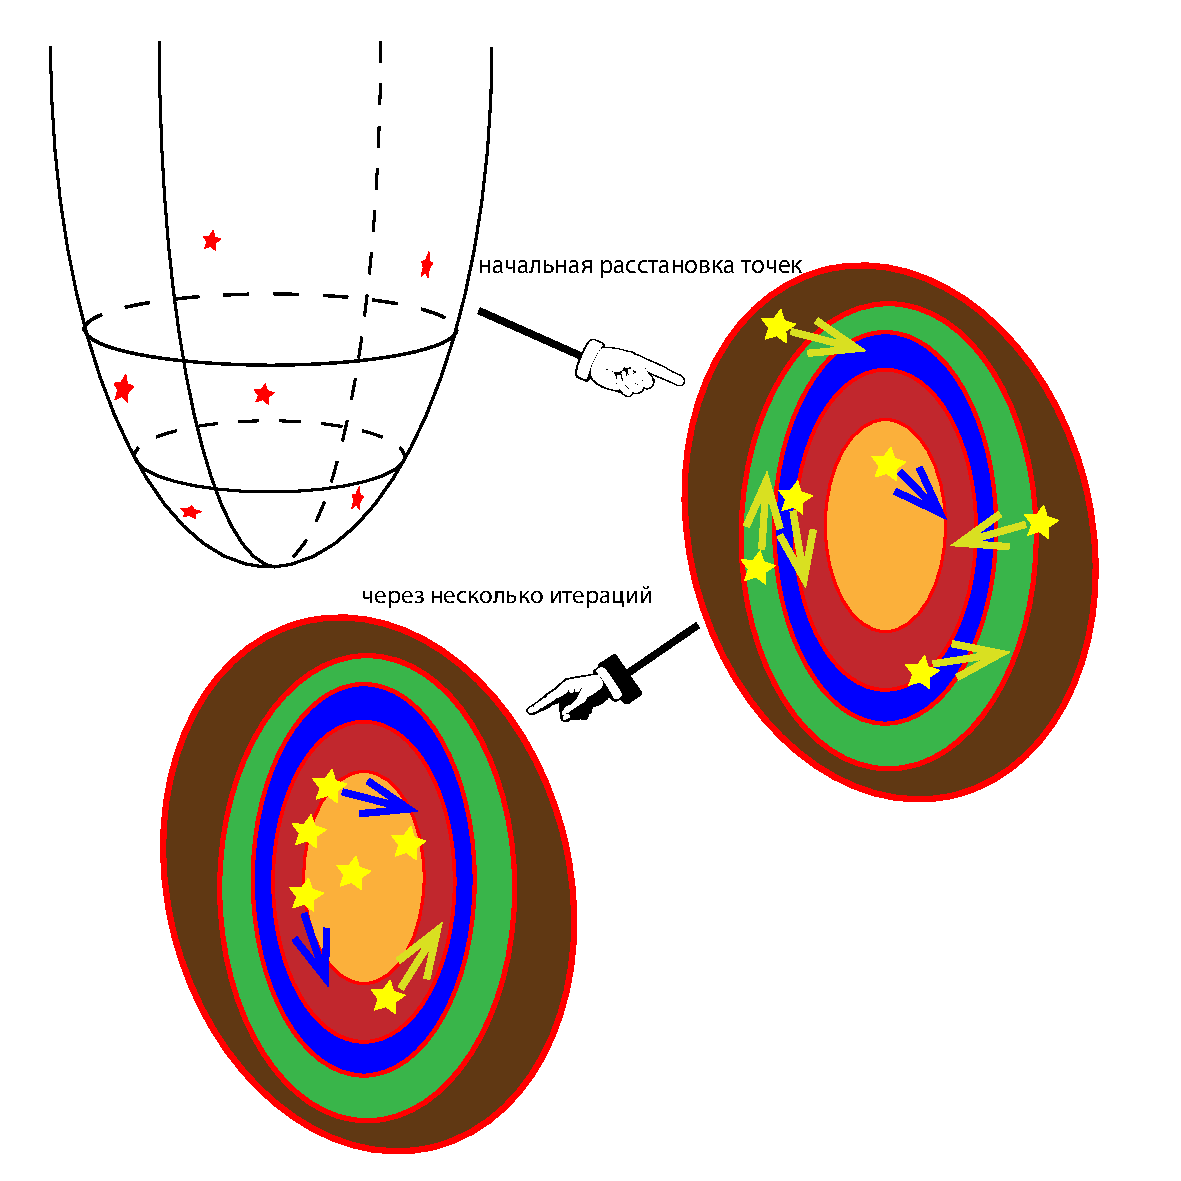
\includegraphics[width=0.6\linewidth]{parab.pdf}}
  \caption{Идея работы метода роя частиц для случая функции двух переменных с единственным минимумом}
  \label{parab}
\end{figure}

\section{Устойчивость алгоритма 2}
Минимизацию функционала (\ref{func}) путём решения системы (\ref{sist}) тяжело адекватно (относительно временных ресурсов) проверить на устойчивость,
используя алгоритм, подобный ультрагибридному для решения ОЗГ, поскольку тогда для каждой размерности придётся заново высчитывать матрицы $D_1^{-1}, D_2^{-1}$.
К счастью, алгоритм роя частиц легко подкорректировать под увеличение размерности задачи, вдобавок он сам по себе гарантирует невозрастание невязки.

На рисунках \ref{s1}-\ref{s4} представлены пары графиков зависимости погрешности аппроксимации от числа $k$ использованных точек $z_1,\dots, z_k$.
На верхнем графике показаны значения для $||u - \tilde{u} ||$ (целевая погрешность), на нижнем --- $F({\bf c},{\bf d})$.

Из графиков видно, что погрешность $F$, как правило, монотонно убывает, пока резко не снизится до достаточно малого значения, ниже которого уже не сможет опуститься.
При этом неубывание $F$ не имеет заметного влияния на поведение $||u - \tilde{u} ||$, то есть алгоритм 2 тоже неустойчивый.

\begin{figure}[h!]
  \center{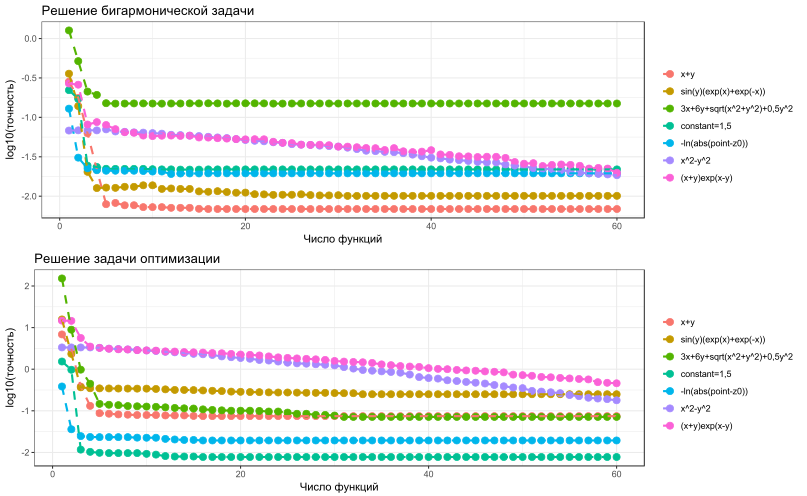
\includegraphics[width=\linewidth]{S1.pdf}}
  \caption{Результат алгоритма 2 для круга}
  \label{s1}
\end{figure}
\begin{figure}[h!]
  \center{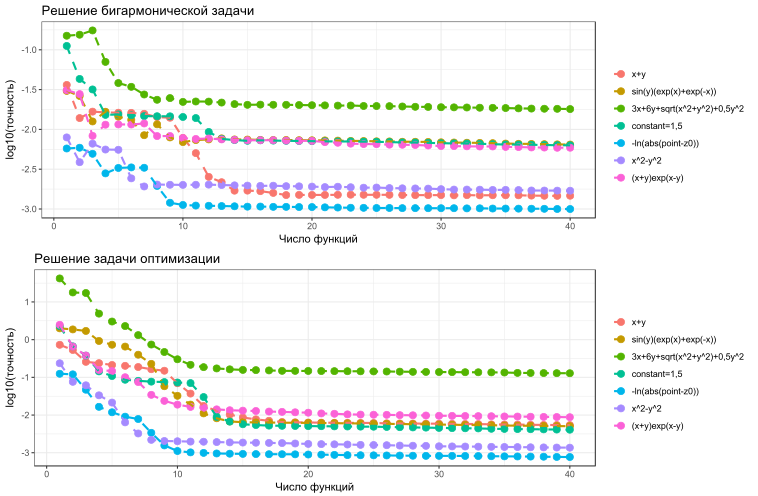
\includegraphics[width=\linewidth]{S2.pdf}}
  \caption{Результат алгоритма 2 для треугольника}
  \label{s2}
\end{figure}
\begin{figure}[h!]
  \center{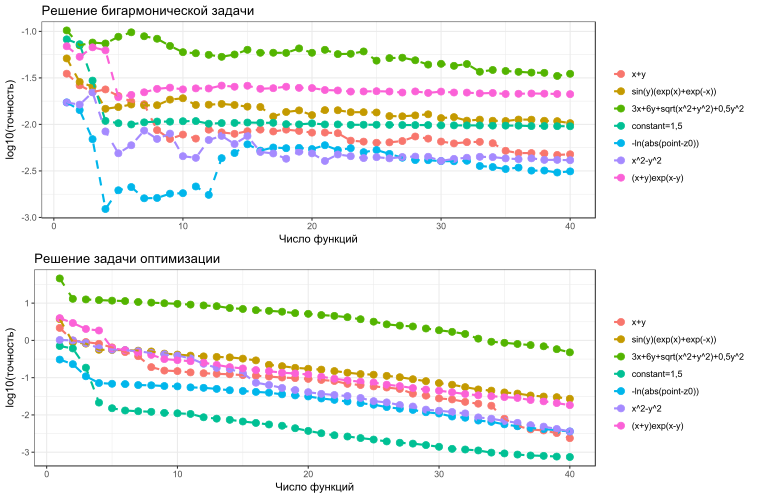
\includegraphics[width=\linewidth]{S3.pdf}}
  \caption{Результат алгоритма 2 для квадрата}
  \label{s3}
\end{figure}
\begin{figure}[h!]
  \center{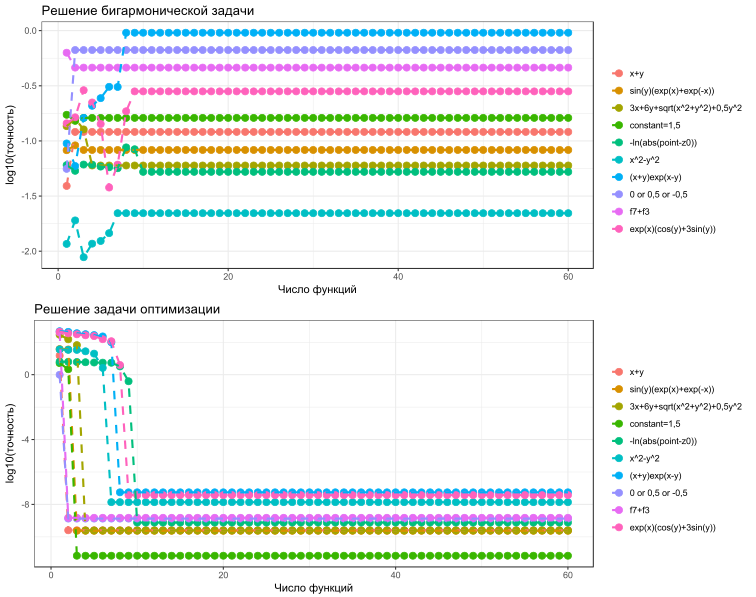
\includegraphics[width=\linewidth]{S4.pdf}}
  \caption{Результат алгоритма 2 для острия}
  \label{s4}
\end{figure}

\begin{figure}[h!]
  \center{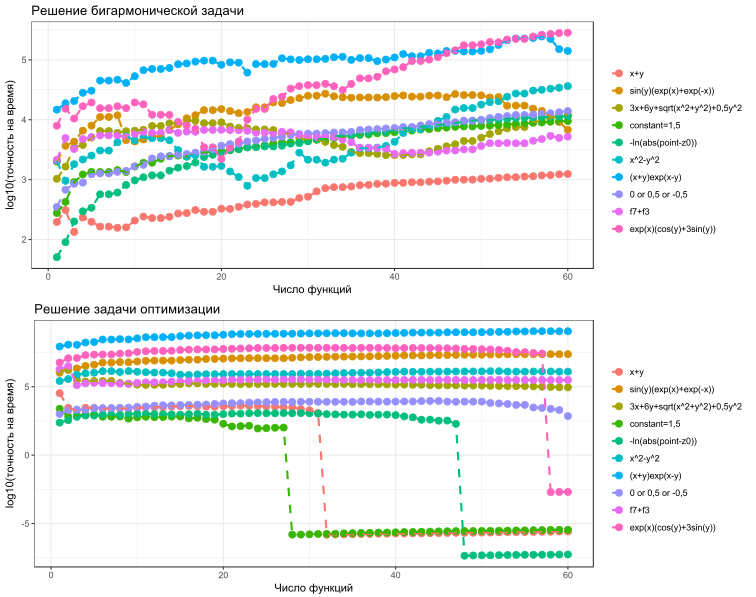
\includegraphics[width=\linewidth]{S5.pdf}}
  \caption{Произведение погрешности на время вычислений для круга}
  \label{s5}
\end{figure}

\section{Сравнение алгоритмов 1 и 2}
Алгоритм 1 имеет два очевидных недостатка:
\begin{enumerate}
  \item В глобальном смысле функция $u$ зависит от дополнительного параметра --- поверхности $L$, --- поэтому определяется неоднозначно, причём, как ранее было показано,
  неизвестно заранее, какая именно поверхность $L$ будет оптимальной и существует ли она вообще.
  \item Итоговая функция $u$ выражается не через комбинацию функций, а как сумма интегралов, причём интегралов с особенностями, что означает наличие значительных погрешностей либо сильные требования к компьютерным ресурсам.  
\end{enumerate}
При этом алгоритм 2 тоже не является устойчивым, что создаёт сомнения, следует ли вообще как-то сравнивать оба алгоритма.
Тем не менее, такое сравнение дало интересные результаты (рисунки \ref{bg1}-\ref{bg2}).

\begin{figure}[h]
  \begin{minipage}[h]{\linewidth}
  \center{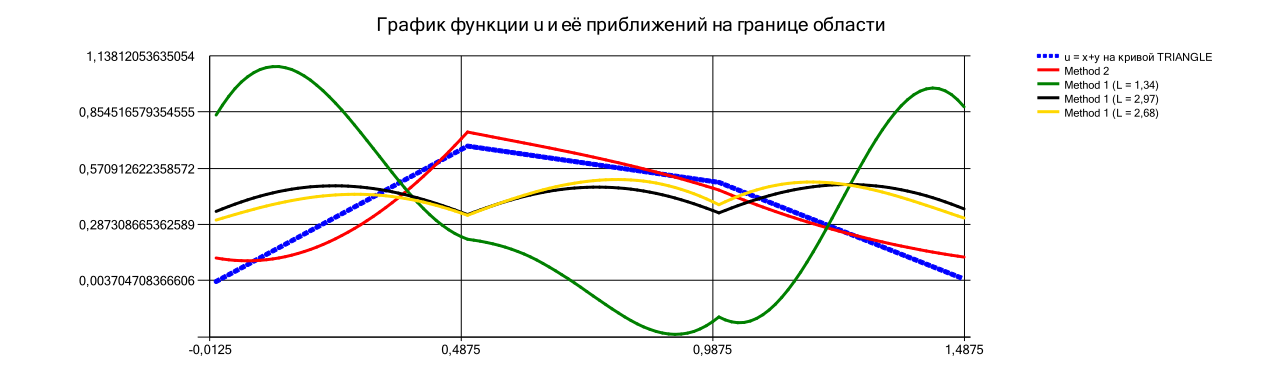
\includegraphics[width=0.95\linewidth]{big1.pdf}}
  \end{minipage}
  \vfill
  \begin{minipage}[h]{\linewidth}
  \center{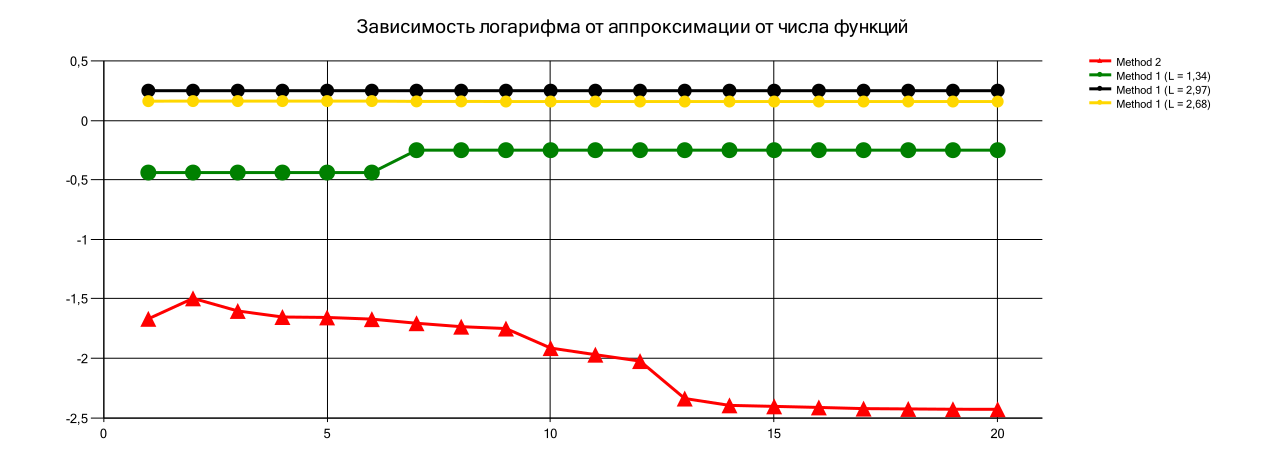
\includegraphics[width=0.95\linewidth]{pig1.pdf}}
  \end{minipage}
  \caption{Результат работы алгоритмов 1 и 2 для функции $f_1$}
  \label{bg1}
  \end{figure}

  \begin{figure}[h]
    \begin{minipage}[h]{\linewidth}
    \center{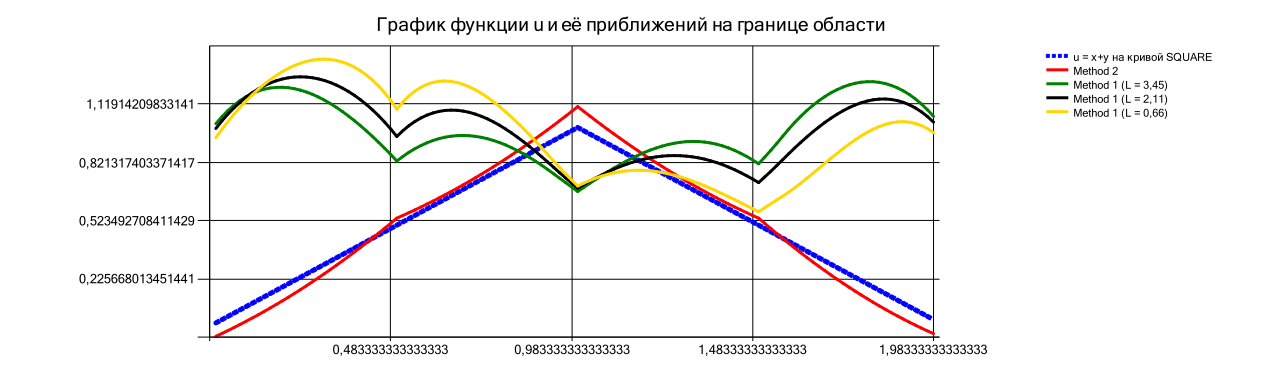
\includegraphics[width=0.95\linewidth]{big2.pdf}}
    \end{minipage}
    \vfill
    \begin{minipage}[h]{\linewidth}
    \center{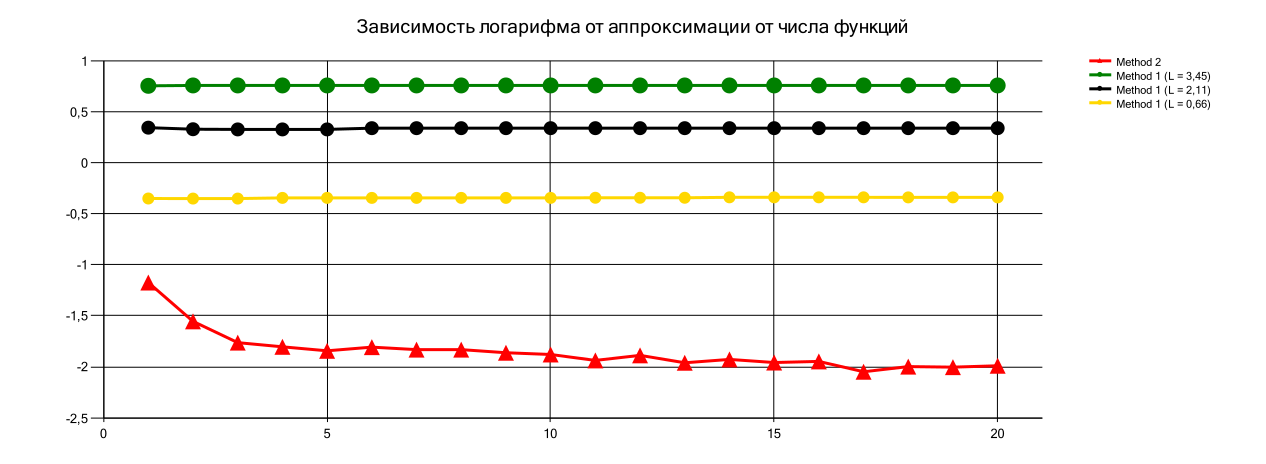
\includegraphics[width=0.95\linewidth]{pig2.pdf}}
    \end{minipage}
    \caption{Результат работы алгоритмов 1 и 2 для функции $f_1$}
    \label{ris:image1}
    \end{figure}

    \begin{figure}[h]
      \begin{minipage}[h]{\linewidth}
      \center{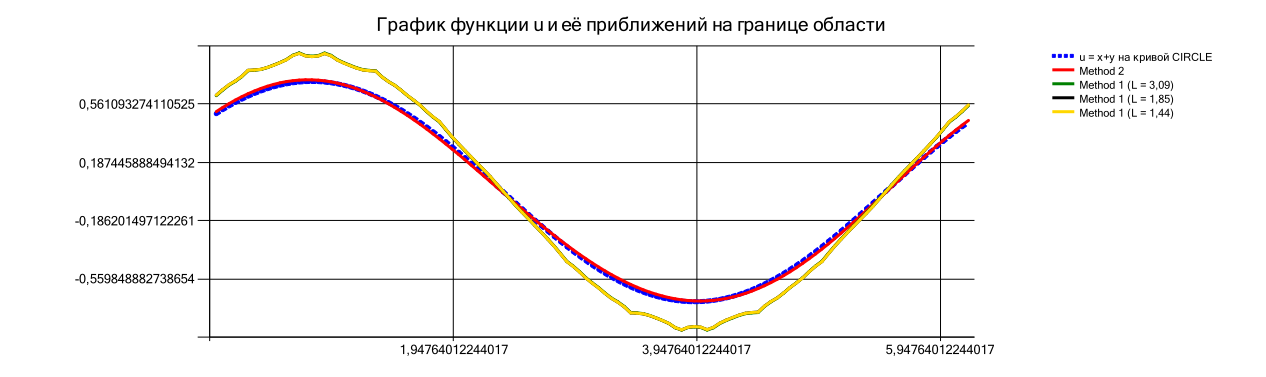
\includegraphics[width=0.95\linewidth]{big3.pdf}}
      \end{minipage}
      \vfill
      \begin{minipage}[h]{\linewidth}
      \center{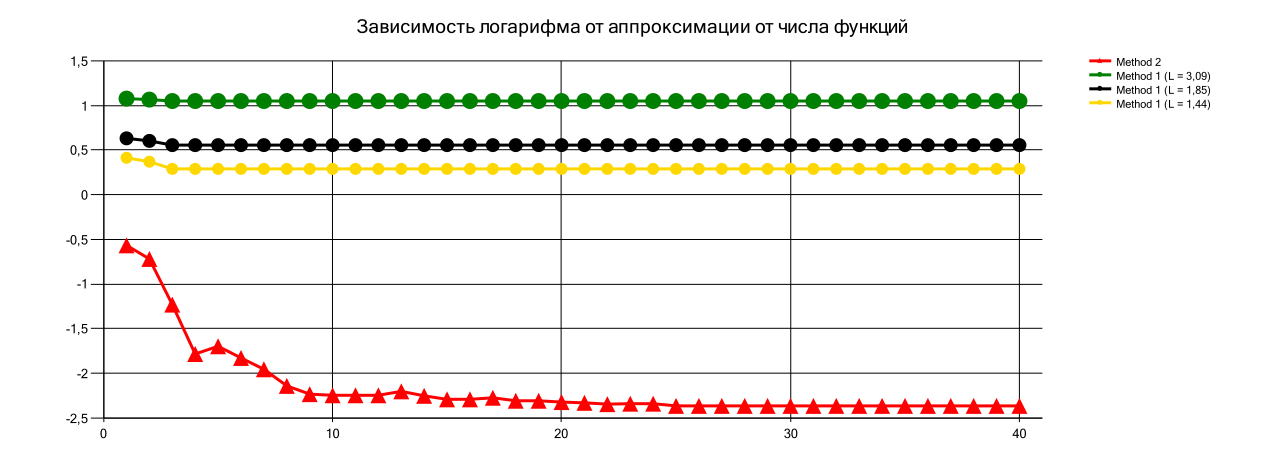
\includegraphics[width=0.95\linewidth]{pig3.pdf}}
      \end{minipage}
      \caption{Результат работы алгоритмов 1 и 2 для функции $f_1$}
      \label{ris:image1}
      \end{figure}

      \begin{figure}[h]
        \begin{minipage}[h]{\linewidth}
        \center{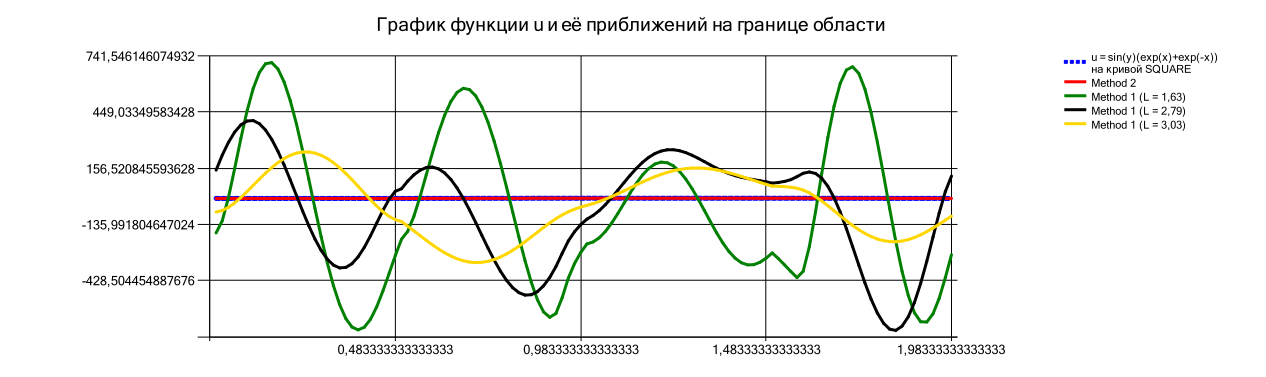
\includegraphics[width=0.95\linewidth]{big4.pdf}}
        \end{minipage}
        \vfill
        \begin{minipage}[h]{\linewidth}
        \center{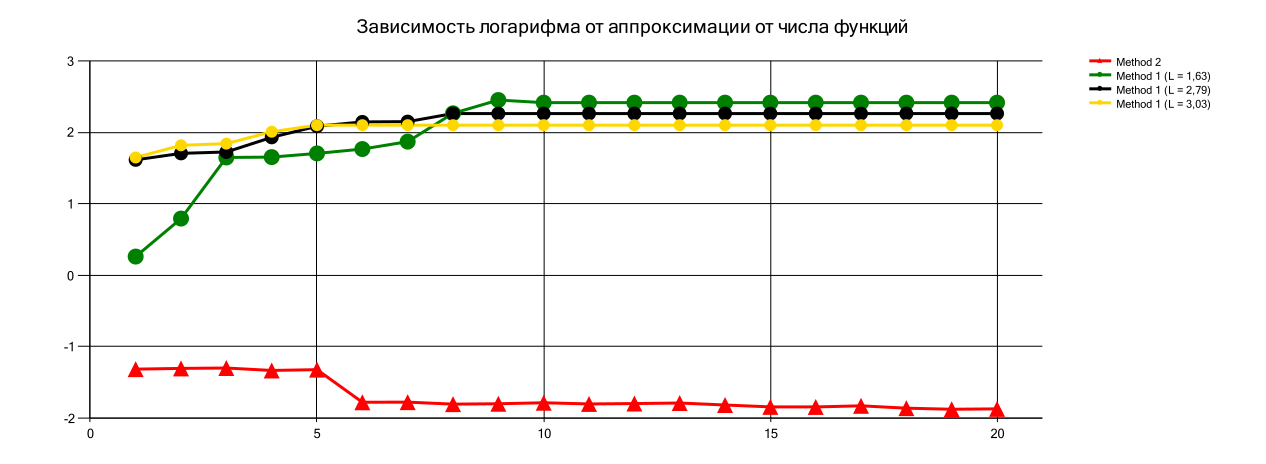
\includegraphics[width=0.95\linewidth]{pig4.pdf}}
        \end{minipage}
        \caption{Результат работы алгоритмов 1 и 2 для функции $f_2$}
        \label{ris:image1}
        \end{figure}

        \begin{figure}[h]
          \begin{minipage}[h]{\linewidth}
          \center{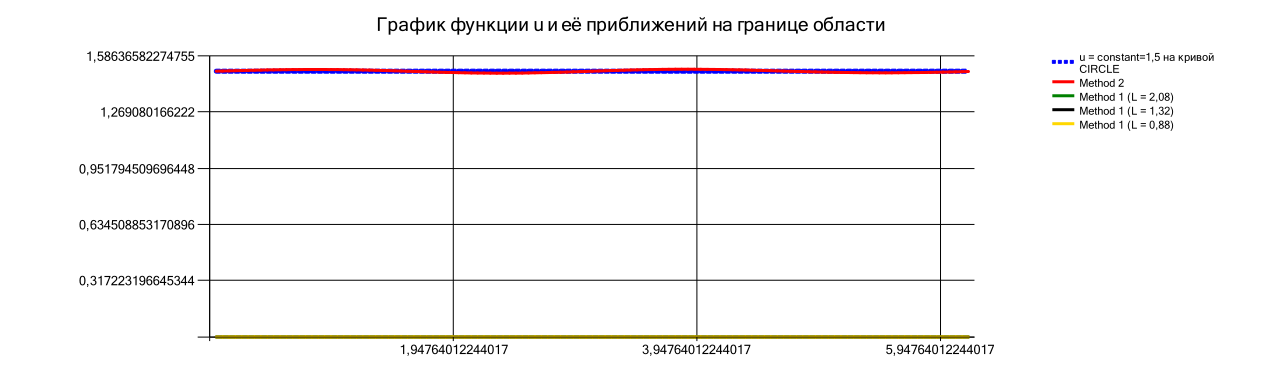
\includegraphics[width=0.95\linewidth]{big5.pdf}}
          \end{minipage}
          \vfill
          \begin{minipage}[h]{\linewidth}
          \center{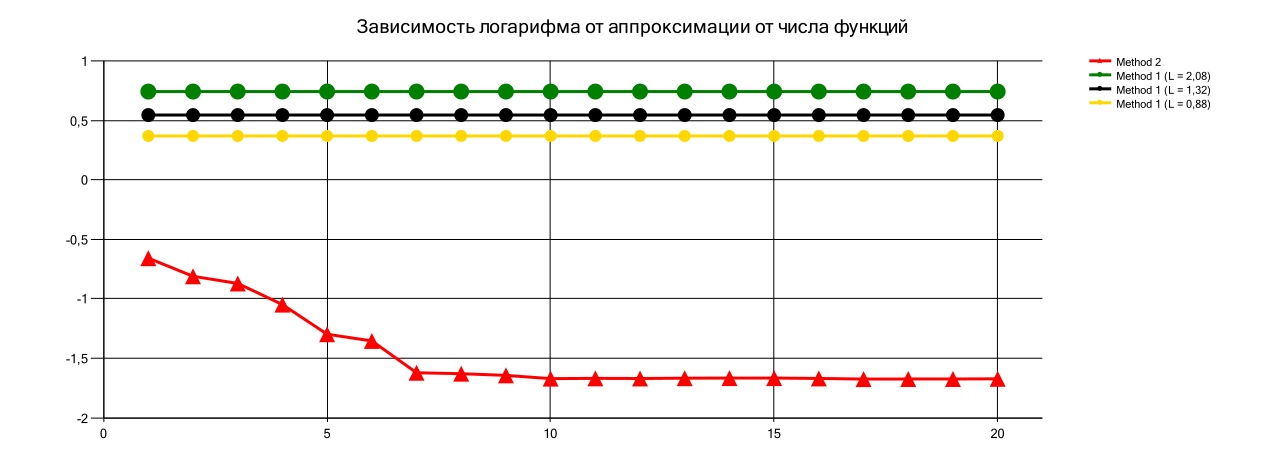
\includegraphics[width=0.95\linewidth]{pig5.pdf}}
          \end{minipage}
          \caption{Результат работы алгоритмов 1 и 2 для функции $f_4$}
          \label{ris:image1}
          \end{figure}

          \begin{figure}[h]
            \begin{minipage}[h]{\linewidth}
            \center{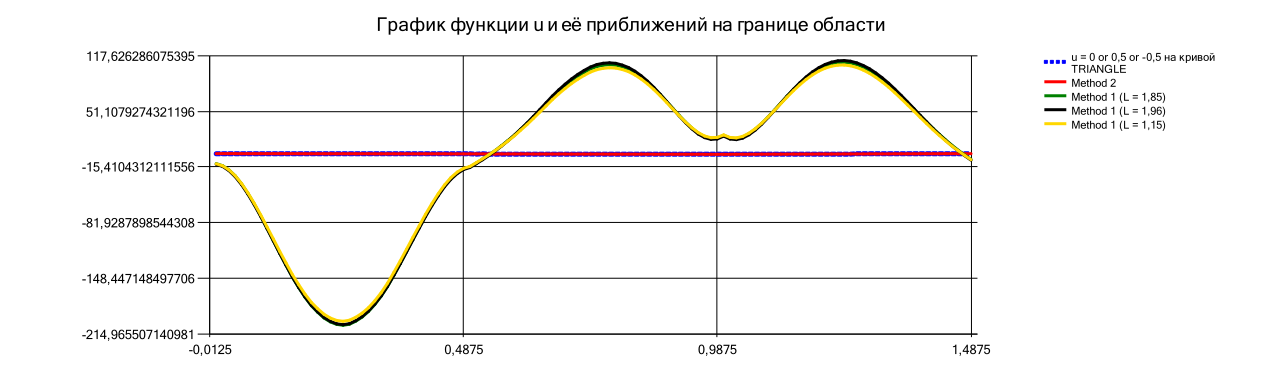
\includegraphics[width=0.95\linewidth]{big6.pdf}}
            \end{minipage}
            \vfill
            \begin{minipage}[h]{\linewidth}
            \center{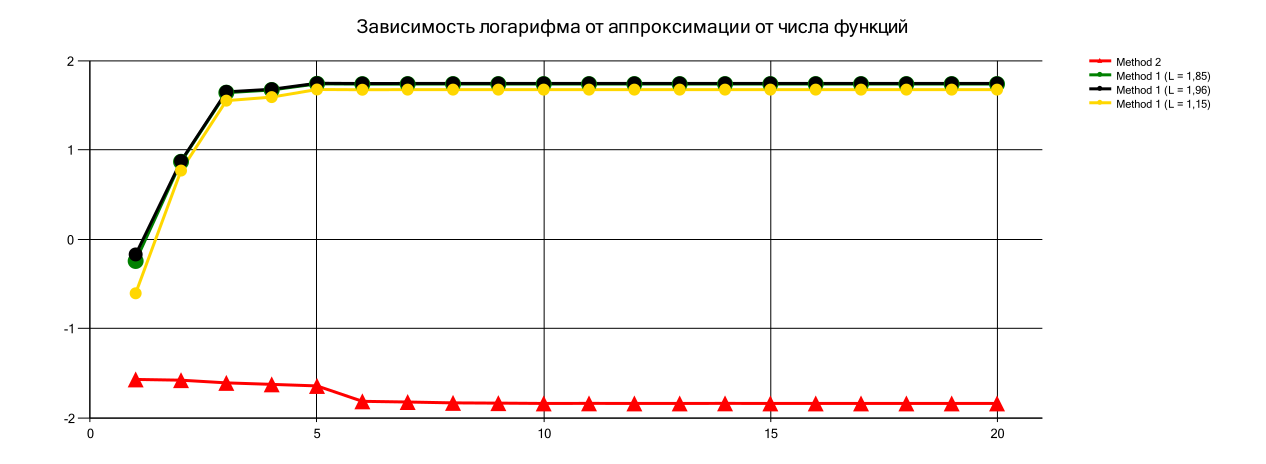
\includegraphics[width=0.95\linewidth]{pig6.pdf}}
            \end{minipage}
            \caption{Результат работы алгоритмов 1 и 2 для функции $f_7$}
            \label{ris:image1}
            \end{figure}

            \begin{figure}[h!]
              \center{\includegraphics[width=\linewidth]{bf1.pdf}}
              \caption{Результат работы алгоритмов 1 и 2 для функции $f_1$}
              \label{s1}
            \end{figure}

            \begin{figure}[h!]
              \center{\includegraphics[width=\linewidth]{bf1b.pdf}}
              \caption{Результат работы алгоритмов 1 и 2 для функции $f_2$}
              \label{s1}
            \end{figure}

            \begin{figure}[h!]
              \center{\includegraphics[width=\linewidth]{bf1b2.pdf}}
              \caption{Результат работы алгоритмов 1 и 2 для функции $f_1$}
              \label{s1}
            \end{figure}

            \begin{figure}[h!]
              \center{\includegraphics[width=\linewidth]{bf4.pdf}}
              \caption{Результат работы алгоритмов 1 и 2 для функции $f_4$}
              \label{s1}
            \end{figure}

            \begin{figure}[h!]
              \center{\includegraphics[width=\linewidth]{bf4b.pdf}}
              \caption{Результат работы алгоритмов 1 и 2 для функции $f_4$}
              \label{s1}
            \end{figure}

            \begin{figure}[h!]
              \center{\includegraphics[width=\linewidth]{bf4b2.pdf}}
              \caption{Результат работы алгоритмов 1 и 2 для функции $f_4$}
              \label{bg2}
            \end{figure}


Просмотрев все тестовые графики, я сделал следующие выводы об эффективности алгоритмов 1 и 2:
\begin{enumerate}
  \item {\itУстойчивость обоих алгоритмов в каждой конкретной бигармонической задаче зависит от выбора точек $z_1, \dots, z_k$}, которые в общем случае выбираются с некоторой долей случайности. При этом {\itмежду устойчивостью алгоритма 1 и алгоритма 2 не наблюдаётся зависимости}.
  \item {\itНесмотря на неустойчивость в общем случае, алгоритм 2 способен решать бигармоническую задачу с некоторой приемлемой точностью, покуда алгоритм 1 такой точности не достигает}.
  \item {\itКонечное решение задачи алгоритмом 1 не сильно зависит от поверхности $L$, поскольку через некоторое число шагов при любой $L$ погрешность начинает вести себя одинаково} (обретает значения, очень близкие к константе, недостаточно малой для приемлемого решения задачи). И хоть на выходе всегда будут немного разные функции, искомую функцию они приближают одинаково плохо.
  \item {\itФункция, найденная алгоритмом 2, почти повторяет поведение искомой функции, а для алгоритма 1 это не так}.
\end{enumerate}

\end{document}